\section{heading 1: my chapter 1}

Heading 1 is the style you should use for the following headings in your thesis: List of Tables, List of Figures (List of Abbreviations, Schemes, and so on), Chapter titles, References, and Appendix titles. If you are writing in APA style, note that the titles formatted as Heading 1 do not count as an APA heading.  

I want to cite something here \parencite{zuo2019standing}. I want to want to try cite~\textcite{zuo2019standing} with in-line style.

\subsection{heading 2: Use for Your broadest Subheading Level, Centered, Bold, Title Case}

Heading 2 is the first major subheading style. If you are writing in APA style, this heading corresponds to a Level 1 APA heading.  

\subsubsection{heading 3: Use for Your Next Heading Level, Left-aligned, Bold, Title Case}

Heading 3 is the second major subheading style. If you are writing in APA style, this heading corresponds to a Level 2 APA heading. 

\paragraph{Heading 4: This Heading is Left-aligned, Boldface Italics, Title Case}
This is an additional heading level, should your thesis require this level of specificity.

Let me add a figure here~\cref{fig:1}:
\begin{figure}[h]
    \centering
    \captionsetup{width=0.6\linewidth} %% change width to adjust the caption alignment
    \caption{Old capital museum}
    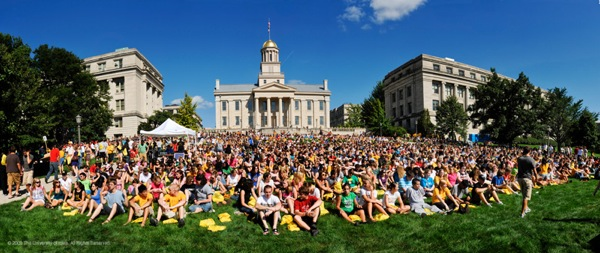
\includegraphics[width=0.6\columnwidth]{fig1}
    \label{fig:1}
\end{figure}
